
\documentclass[11pt]{book}


% ***************************************************************************************************
% Ustawienia języka
% ***************************************************************************************************

% Podstawowe ustawienia języka, według którego {}ormatowany będzie dokument
\usepackage[polish]{babel}

% Pakiet babel dla polskiego języka powoduje konflikt z pakietem amssymb.
% Polecenie '\lll' definiują oba pakiety - porządana jest druga definicja.
\let\lll\undefined

% W przypadku wielojęzykowości ustawia główny język dokumentu
\selectlanguage{polish}

% Kodowanie dokumentu
\usepackage[utf8]{inputenc}

% Dowolny rozmiar czcionek, kodowanie znaków
\usepackage{lmodern}

% Polskie wcięcia akapitów
\usepackage{indentfirst}

% Polskie łamanie wyrazów
\usepackage[plmath]{polski}

% Przecinek w wyrażeniach matematycznych zamiast kropki
\usepackage{icomma}

% Polskie formatowanie typograficzne
\frenchspacing

% Zapewnia liczne usprawnienia wyświetlania i organizacji matematycznych formuł. 
\usepackage{amsmath}
\usepackage{float}

% Wprowadza rozszerzony zestaw symboli m.in. \leadsto
\usepackage{amssymb}

% Dodatkowa, ,,kręcona'' czcionka matematyczna
\usepackage{mathrsfs}

% Dodatkowe wsparcie dla środowiska mathbb, które nie wspiera domyślnie cyfr (\mathbb{})
\usepackage{bbold}

% Fixes/improves amsmath
\usepackage{mathtools}


% ***************************************************************************************************
% Kolory  
% ***************************************************************************************************

% Umożliwia kolorowanie poszczególnych komórek tabeli
\usepackage[table]{xcolor}% http://ctan.org/pkg/

% Umożliwia łatwą zmianę koloru linii w tabeli
\usepackage{tabu}

% Umożliwia rozszerzoną kontrolę nad kolorami.
\usepackage{xcolor}

% Definicje kolorów
\definecolor{lgray}{HTML}{9F9F9F}
\definecolor{dgray}{HTML}{5F5F5F}
% lgray				-	nazwa nowo zdefiniowanego koloru
% HTML				-	model kolorów
% CCCCCC			-	wartość koloru zgodna z modelem

% ***************************************************************************************************
% Algorytmy 
% ***************************************************************************************************

% Udostępnia środowisko do konstruowania pseudokodów
\usepackage[ruled,vlined,linesnumbered,longend,algochapter]{algorithm2e}
% ruled	- poziome kreski na początku i końcu algorytmu, podpis na górze oddzielony również kreską poziomą
% vlined - pionowe kreski łączące początek polecenia z jego końcem
% linesnumbered	- numerowanie kolejnych wierszy algorytmu
% longend - długie końcówki np. ifend, forend itd.
% algochapter - numeracja z rozdziałami

% Zamiana nazwy środowiska z domyślnej "Algorithm X" na "Pseudokod X"
\newenvironment{pseudokod}[1][htb]{
	\renewcommand{\algorithmcfname}{Pseudokod}
	\begin{algorithm}[#1]%
	}{
\end{algorithm}
}

% Zmiana rozmiaru komentarzy
\newcommand\algcomment[1]{
	\footnotesize{#1}
}

% Ustawienie zadanego stylu dla komentarzy
\SetCommentSty{algcomment}

% Wyśrodkowana tylda
\usepackage{textcomp}%
\newcommand{\textapprox}{\raisebox{0.5ex}{\texttildelow}}

% Listowanie kodów źródłowych
\usepackage{listings} 
\renewcommand{\lstlistingname}{Kod źródłowy} % Polska nazwa listingu

% Definicje pecjalnych znaków, które nie są obsługiwane w środowisku listing
\lstset{literate=
	{ż}{{\.{z}}}1	{ź}{{\'{z}}}1
	{ć}{{\'{c}}}1	{ń}{{\'{n}}}1
	{ą}{{\c a}}1	{ś}{{\'{s}}}1
	{ł}{{\l}}1		{ę}{{\c{e}}}1
	{ó}{{\'{o}}}1	{á}{{\'a}}1
	{é}{{\'e}}1		{í}{{\'i}}1
	{ó}{{\'o}}1		{ú}{{\'u}}1
	{ù}{{\`u}}1		{Á}{{\'A}}1
	{É}{{\'E}}1		{Í}{{\'I}}1
	{Ó}{{\'O}}1		{Ú}{{\'U}}1
	{à}{{\`a}}1		{è}{{\'e}}1
	{ì}{{\`i}}1		{ò}{{\`o}}1
	{ò}{{\`o}}1		{À}{{\`A}}1
	{È}{{\'E}}1		{Ì}{{\`I}}1
	{Ò}{{\`O}}1		{Ò}{{\`O}}1
	{ä}{{\"a}}1		{ë}{{\"e}}1
	{ï}{{\"i}}1		{ö}{{\"o}}1
	{ü}{{\"u}}1		{Ä}{{\"A}}1
	{Ë}{{\"E}}1		{Ï}{{\"I}}1
	{Ö}{{\"O}}1		{Ü}{{\"U}}1
	{â}{{\^a}}1		{ê}{{\^e}}1
	{î}{{\^i}}1		{ô}{{\^o}}1
	{û}{{\^u}}1		{Â}{{\^A}}1
	{Ê}{{\^E}}1		{Î}{{\^I}}1
	{Ô}{{\^O}}1		{Û}{{\^U}}1
	{œ}{{\oe}}1		{Œ}{{\OE}}1
	{æ}{{\ae}}1		{Æ}{{\AE}}1
	{ß}{{\ss}}1		{ç}{{\c c}}1
	{Ç}{{\c C}}1	{ø}{{\o}}1
	{å}{{\r a}}1	{Å}{{\r A}}1
	{€}{{\EUR}}1	{£}{{\pounds}}1
}

% ***************************************************************************************************
% Marginesy 
% ***************************************************************************************************

% Ustawienia rozmiarów stron i ich marginesów
\usepackage[headheight=18pt, top=25mm, bottom=25mm, left=25mm, right=25mm]{geometry}
% headheight		-	wysokość tytułów
% top				-	margines górny
% bottom			-	margines dolny
% left				-	margines lewy
% right				-	margines prawy

% Usunięcie górnego marginesu dla środowisk
\makeatletter
\setlength\@fptop{0\p@}	
\makeatother

% ***************************************************************************************************
% Styl 
% ***************************************************************************************************

% Definiuje środowisko 'titlingpage', które zapewnia pełną kontrolę nad układem strony tytułowej.
\usepackage{titling}


% Umożliwia modyfikowanie stylu spisu treści
\usepackage{tocloft}	

\tocloftpagestyle{tableOfContentStyle}

% Definiowanie własnych stylów nagłówków i/lub stopek
\usepackage{fancyhdr}

% Domyślny styl dla pracy 
\fancypagestyle{custom}{
	\fancyhf{}									% wyczyść stopki i nagłówki
	\fancyhead[RO]{								% Prawy, nieparzysty nagłówek
		\hrulefill \hspace{16pt} \large Rozdział \thechapter
		\put(-472.1, 12.1){%
			\makebox(0,0)[l]{%
				
\includegraphics[width=0.05\textwidth]{pwr-logo}
			}
		}
		\put(-443,5.5){%
			\makebox(0,0)[l]{%
				\small Politechnika Wrocławska
			}
		}
	}
	\fancyhead[LE]{								% Lewy, parzysty nagłówek
		\large Rozdział \thechapter \hspace{16pt} \hrulefill 
		\put(-22, 12.1){%
			\makebox(0,0)[l]{%
				
\includegraphics[width=0.05\textwidth]{wppt-logo}
			}
		}
		\put(-220,5.5){%
			\makebox(0,0)[l]{%
				\small Wydział Podstawowych Problemów Techniki
			}
		}
	}
	\fancyfoot[LE,RO]{							% Stopki
		\thepage
	}
	\renewcommand{\headrulewidth}{0pt}			% Grubość linii w nagłówku
	\renewcommand{\footrulewidth}{0.2pt}		% Grubość linii w stopce
}


% Domyślny styl dla bibliografii
\fancypagestyle{bibliographyStyle}{
	\fancyhf{}									% wyczyść stopki i nagłówki
	\fancyhead[RO]{								% Prawy, nieparzysty nagłówek
		\hrulefill \hspace{16pt} \large Dodatek \thechapter
		\put(-472.1, 12.1){%
			\makebox(0,0)[l]{%
				
\includegraphics[width=0.05\textwidth]{pwr-logo}
			}
		}
		\put(-443,5.5){%
			\makebox(0,0)[l]{%
				\small Politechnika Wrocławska
			}
		}
	}
	\fancyhead[LE]{								% Lewy, parzysty nagłówek
		\large Bibliografia \hspace{16pt} \hrulefill 
		\put(-22, 12.1){%
			\makebox(0,0)[l]{%
				
\includegraphics[width=0.05\textwidth]{wppt-logo}
			}
		}
		\put(-210,5.5){%
			\makebox(0,0)[l]{%
				\small Wydział Podstawowych Problemów Techniki
			}
		}
	}
	\fancyfoot[LE,RO]{							% Stopki
		\thepage
	}
	\renewcommand{\headrulewidth}{0pt}			% Grubość linii w nagłówku
	\renewcommand{\footrulewidth}{0.2pt}		% Grubość linii w stopce
}

% Domyślny styl dla dodatków
\fancypagestyle{appendixStyle}{
	\fancyhf{}									% wyczyść stopki i nagłówki
	\fancyhead[RO]{								% Prawy, nieparzysty nagłówek
		\hrulefill \hspace{16pt} \large Dodatek \thechapter
		\put(-472.1, 12.1){%
			\makebox(0,0)[l]{%
				
\includegraphics[width=0.05\textwidth]{pwr-logo}
			}
		}
		\put(-443,5.5){%
			\makebox(0,0)[l]{%
				\small Politechnika Wrocławska
			}
		}
	}
	\fancyhead[LE]{								% Lewy, parzysty nagłówek
		\large Dodatek \thechapter \hspace{16pt} \hrulefill 
		\put(-22, 12.1){%
			\makebox(0,0)[l]{%
				
\includegraphics[width=0.05\textwidth]{wppt-logo}
			}
		}
		\put(-210,5.5){%
			\makebox(0,0)[l]{%
				\small Wydział Podstawowych Problemów Techniki
			}
		}
	}
	\fancyfoot[LE,RO]{							% Stopki
		\thepage
	}
	\renewcommand{\headrulewidth}{0pt}			% Grubość linii w nagłówku
	\renewcommand{\footrulewidth}{0.2pt}		% Grubość linii w stopce
}

% Osobny styl dla stron zaczynających rozdział/spis treści itd. (domyślnie formatowane jako "plain")
\fancypagestyle{chapterBeginStyle}{
	\fancyhf{}%
	\fancyfoot[LE,RO]{
		\thepage
	}
	\renewcommand{\headrulewidth}{0pt}
	\renewcommand{\footrulewidth}{0.2pt}
}

% Styl dla pozostałych stron spisu treści
\fancypagestyle{tableOfContentStyle}{
	\fancyhf{}%
	\fancyfoot[LE,RO]{
		\thepage
	}
	\renewcommand{\headrulewidth}{0pt}
	\renewcommand{\footrulewidth}{0.2pt}
}

% Formatowanie tytułów rozdziałów i/lub sekcji
\usepackage{titlesec}

% Formatowanie tytułów rozdziałów
\titleformat{\chapter}[hang]					% kształt
{
	\vspace{-10ex}
	\Huge
	\bfseries
}												% formatowanie tekstu modyfikowanego elementu
{}												% etykieta występująca przed tekstem modyfikowanego elementu, niewidoczna w spisie treści
{
	10pt
}												% odstęp formatowanego tytułu od lewego marginesu/etykiety
{
	\Huge
	\bfseries
}												% formatowanie elementów przed modyfikowanym tytułem
[
\vspace{2ex}
%\rule{\textwidth}{0.4pt}
%\vspace{-4ex}
]												% dodatkowe formatowanie stosowane poniżej modyfikowanego tytułu


% Formatowanie tytułów sekcji
\titleformat{\section}[hang]					% kształt
{
	\vspace{2ex}
%	\titlerule\vspace{1ex}
	\Large\bfseries
}												% formatowanie tekstu modyfikowanego elementu
{
	\thesection									% etykieta występująca przed tekstem modyfikowanego elementu, niewidoczna w spisie treści
}
{
	0pt
}												% odstęp formatowanego tytułu od lewego marginesu/etykiety
{
	\Large
	\bfseries
}												% formatowanie elementów przed modyfikowanym tytułem

% ***************************************************************************************************
% Linki
% ***************************************************************************************************

% Umożliwia wstawianie hiperłączy do dokumentu
\usepackage{hyperref}							% Aktywuje linki

\hypersetup{
	colorlinks	=	true,					% Koloruje tekst zamiast tworzyć ramki.
	linkcolor		=	blue,					% Kolory: referencji,
        citecolor		=	blue,					% cytowań,
	urlcolor		=	blue					% hiperlinków.
}

% Do stworzenia hiperłączy zostanie użyta ta sama (same) czcionka co dla reszty dokumentu
\urlstyle{same}




% ***************************************************************************************************
% Linki
% ***************************************************************************************************

% Umożliwia zdefiniowanie własnego stylu wyliczeniowego
\usepackage{enumitem}

% Nowa lista numerowana z trzema poziomami
\newlist{myitemize}{itemize}{3}

% Definicja wyglądu znacznika pierwszego poziomu
\setlist[myitemize,1]{
	label		=	\textbullet,
	leftmargin	=	4mm}

% Definicja wyglądu znacznika drugiego poziomu
\setlist[myitemize,2]{
	label		=	$\diamond$,
	leftmargin	=	8mm}

% Definicja wyglądu znacznika trzeciego poziomu
\setlist[myitemize,3]{
	label		=	$\diamond$,
	leftmargin	=	12mm
}

% ***************************************************************************************************
% Inne pakiety
% ***************************************************************************************************

% Dołączanie rysunków
\usepackage{graphicx}

% Figury i przypisy
\usepackage{caption}
\usepackage{subcaption}

% Umożliwia tworzenie przypisów wewnątrz środowisk
\usepackage{footnote}

% Umożliwia tworzenie struktur katalogów
\usepackage{dirtree}

% Rozciąganie komórek tabeli na wiele wierszy
\usepackage{multirow}

% Precyzyjne obliczenia szerokości/wysokości dowolnego fragmentu wygenerowanego przez LaTeX
\usepackage{calc}

% ***************************************************************************************************
% Matematyczne skróty
% ***************************************************************************************************

% Skrócony symbol liczb rzeczywistych
\newcommand{\RR}{\mathbb{R}}

% Skrócony symbol liczb naturalnych
\newcommand{\NN}{\mathbb{N}}

% Skrócony symbol liczb wymiernych
\newcommand{\QQ}{\mathbb{Q}}

% Skrócony symbol liczb całkowitych
\newcommand{\ZZ}{\mathbb{Z}}

% Skrócony symbol logicznej implikacji
\newcommand{\IMP}{\rightarrow}

% Skrócony symbol  logicznej równoważności
\newcommand{\IFF}{\leftrightarrow}

% ***************************************************************************************************
% Środowiska
% ***************************************************************************************************

% Środowisko do twierdzeń
\newtheorem{theorem}{Twierdzenie}[chapter]

% Środowisko do lematów
\newtheorem{lemma}{Lemat}[chapter]

% Środowisko do przykładów
\newtheorem{example}{Przykład}[chapter]

% Środowisko do wniosków
\newtheorem{corollary}{Wniosek}[chapter]

% Środowisko do definicji
\newtheorem{definition}{Definicja}[chapter]

% Środowisko do dowodów
\newenvironment{proof}{
	\par\noindent \textbf{Dowód.}
}{
\begin{flushright}
	\vspace*{-6mm}\mbox{$\blacklozenge$}
\end{flushright}
}

% Środowisko do uwag
\newenvironment{remark}{
	\bigskip \par\noindent \small \textbf{Uwaga.}
}{
\begin{small}
	\vspace*{4mm}
\end{small}
}

% ***************************************************************************************************
% Słownik
% ***************************************************************************************************

% Prawidłowe dzielenie wyrazów
\hyphenation{wszy-stkich ko-lu-mnę każ-da od-leg-łość
	dzie-dzi-ny dzie-dzi-na rów-nych rów-ny
	pole-ga zmie-nna pa-ra-met-rów wzo-rem po-cho-dzi
	o-trzy-ma wte-dy wa-run-ko-wych lo-gicz-nie
	skreś-la-na skreś-la-ną cał-ko-wi-tych wzo-rów po-rzą-dek po-rząd-kiem
	przy-kład pod-zbio-rów po-mię-dzy re-pre-zen-to-wa-ne
	rów-no-waż-ne bi-blio-te-kach wy-pro-wa-dza ma-te-ria-łów
	prze-ka-za-nym skoń-czo-nym moż-esz na-tu-ral-na cią-gu tab-li-cy
	prze-ka-za-nej od-po-wied-nio}

% ***************************************************************************************************
% Dokument
% ***************************************************************************************************

\frontmatter

\begin{document}

	\begin{titlingpage}
		\vspace*{\fill}
		\begin{center}
			\begin{picture}(300,510)
				\put(11,520){\makebox(0,0)[l]{\large \textsc{Wydział Podstawowych Problemów Techniki}}}
				\put(11,500){\makebox(0,0)[l]{\large \textsc{Politechnika Wrocławska}}}
% Tytuł pracy
				\put(80,320){\Huge \textsc{Framework e-commerce}}
% Autor pracy
				\put(90,200){\makebox(0,0)[l]{\large \textsc{Przemysław Magiera}}}
				\put(90,180){\makebox(0,0)[l]{\large \textsc{Nr indeksu: 229773}}}

				\put(200,100){\makebox(0,0)[l]{\large Praca inżynierska napisana}}
				\put(200,80){\makebox(0,0)[l]{\large pod kierunkiem}}
% dane promotora
				\put(200,60){\makebox(0,0)[l]{\large Wojciecha Macyny}}
				
				\put(115,-70){
\includegraphics[width=0.15\textwidth]{pwr}}
				\put(106,-80){\makebox(0,0)[bl]{\large \textsc{Wrocław 2018}}}
			\end{picture}
		\end{center}	
		\vspace*{\fill}
	\end{titlingpage}
	
        \cleardoublepage
		
	\pagenumbering{Roman}
	\pagestyle{tableOfContentStyle}
	\tableofcontents
	\cleardoublepage
		
	% ***************************************************************************************************
	% Wstęp
	% ***************************************************************************************************
	
	\pagestyle{custom}
	\mainmatter
	
	% ***************************************************************************************************
	% Rodziały
	% ***************************************************************************************************

	\chapter{Wstęp}
\thispagestyle{chapterBeginStyle}
Celem niniejszej pracy dyplomowej jest zaprojektowanie i zaimplementowanie frameworku służącego do usprawnienia implementacji systemów e-commerce. Istnieje wiele rozwiązań tego typu, jednak bardzo duża część z nich nie oferuje satysfakcjonujących parametrów wydajnościowych, przez co platformy oparte o takie frameworki są czesto bardzo powolne, do tego rozwijane od wielu lat wykorzystują stare rozwiązania i technologie. Prowadzi to często do niepotrzebnego skalowania pionowego aplikacji, czyli zwiększania mocy obliczeniowej. Proces ten wiąże się z bardzo dużymi kosztami, szczególnie w przypadku platform handlowych typu B2B. Zdecydowanie lepszym wyjściem okazuje się w takim przypadku jeden z dzisiejszych trendów budowania aplikacji, czyli skalowanie poziome, polegające na dzieleniu aplikacji według zastosowania poszczególnych komponentów, umieszczając niezależne jej części na serwerach dziedzinowych (architektura mikroserwisowa). Taka architektura pozwala na skalowanie tylko konkretnych, najbardziej narażonych na wzmożony ruch, elementów infrastruktury, co skutkuje bardzo dużą oszczędnością w stosunku do aplikacji monolitycznych. Budowa mikroserwisowa nie jest jednak cudownym środkiem na każdego rodzaju problemy dzisiejszych aplikacji internetowych, wiąże się z nim bowiem wiele problemów, jak chociażby integracja i synchronizacja między komponentami lub konieczność administracji bardzo złożonego środowiska. Właśnie ze względu na to ostatnie widzimy dziś tak wiele ofert pracy na stanowisko DevOps (development and operations). Wydaje się dlatego, że architektura monolityczna z oddzieleniem warstwy katalogowej (tej najbardziej obciążonej) jest optymalnym rozwiązaniem problemu implementacji sklepów internetowych.
\newline
Często dewelopment aplikacji idzie w parze z presją czasu, przez co zapomina  się o jakości kodu i rozwiązaniach, które poprawiłyby wydajność i ograniczyły konieczność skalowania. Z zamkniętymi oczami podąża się za schematami i szablonami, aby dostarczyć rozwiązanie jak najszybciej, a nie jak najlepiej. Dlatego właśnie założeniem projektu w ramach pracy jest zaprojektowanie i implementacja frameworku e-commerce spełniającego następujące założenia funkcjonalne:

Praca składa się z czterech rozdziałów. W rozdziale pierwszym omówiono strukturę przedsiębior-
stwa . . . , scharakteryzowano grupy użytkowników oraz przedstawiono procedury związane z obie-
giem dokumentów. Szczegółowo opisano mechanizmy . . . . Przedstawiono uwarunkowania prawne
udostępniania informacji . . . , w ramach . . . .
W rozdziale drugim przedstawiono szczegółowy projekt systemy w notacji UML. Wykorzystano
diagramy . . . . Zawarto w niej w pseudokod algorytmów generowania oraz omówiono jego właściwo-
ści. . . 
\newpage
\section{Słowniczek}
\noindent
\textit{indeksacja} -- proces synchronizacji pomiędzy relacyjną bazą danych, a szybką bazą noSQL, używany w systemie do encji najbardziej narzuconych na duże wykorzystanie. W skrócie: 
\begin{quote}
	\textit{By adding content to an \textbf{index}, we make it searchable by Solr.}\cite{Solr} 
\end{quote}


\noindent
\textit{facet} -- jest to atrybut danej encji, zazwyczaj wyszukiwalny. Używa się ich do implementacji filtrów używanych podczas wyszukiwania. Z dokumentacji Solra:
\begin{quote} \textit{
	Searchers are presented with the indexed terms, along with numerical counts of how many matching documents were found were each term. Faceting makes it easy for users to explore search results, narrowing in on exactly the results they are looking for.
	}\cite{Solr}
\end{quote}


\noindent
\textit{release} -- jest to atrybut danej encji, zazwyczaj wyszukiwalny. Używa się ich do implementacji filtrów używanych podczas wyszukiwania. Z dokumentacji Solra:
\begin{quote} \textit{
		Searchers are presented with the indexed terms, along with numerical counts of how many matching documents were found were each term. Faceting makes it easy for users to explore search results, narrowing in on exactly the results they are looking for.
	}\cite{Solr}
\end{quote}

\noindent
\textit{release} -- nieskopoziomowe udogodnienie w języku Java, pozwalające na operacje i wyświetlanie właściwości klasy Javowej.
\begin{quote} \textit{
		Reflection is a feature in the Java programming language. It allows an executing Java program to examine or "introspect" upon itself, and manipulate internal properties of the program. For example, it's possible for a Java class to obtain the names of all its members and display them.
	}\cite{oracle}
\end{quote}





	\cleardoublepage

	\chapter{Analiza problemu}
\thispagestyle{chapterBeginStyle}
\label{rozdzial1}

W tym rozdziale została przedstawiona analiza zagadnienia. Nakreślono problemy i omówiono proponowane przez system rozwiązania. Omówiono założenia funkcjonalne i niefunkcjonalne samego systemu jak i jego podsystemów.


\section{Charakterystyka problemu}
Aplikacje webowe, a w szczególności systemy e-commerce, są często wolne. Pisane przez niedoświadczonych deweloperów pod presją czasu nie zawsze wychodzą tak jak powinny. Więc jak powinny być napisane? W pierwszej kolejności muszą być dobrze przemyślane, a co za tym idzie ich architektura powinna być przygotowana na rozszerzenia i modyfikacje. Powiedzmy, że mamy sklep internetowy, na bazie którego chcielibyśmy stworzyć jakiś inny sklep. Często jest to niemożliwe ze względu na budowę i obsługę komponentów. Dobrym przykładem na to jest indeksowanie produktów do mechanizmu wyszukującego.
\begin{example}
	W systemie istnieje klasa Product z zadeklarowanymi polami biznesowymi, powiedzmy że klient chce nowe pole o nazwie myCustomField, oczywiście ma być ono wyszukiwalne. Rozszerzamy więc klasę Produkt do MyProdukt i dodajemy pole myCustomField. Mechanizm indeksacji nie ma możliwości wyciągnąć z Produktu pola dotyczącego klasy MyProdukt, ponieważ zaprzeczałoby to zasadom polimorfizmu.
\end{example} 
To tylko konkretny przykład, ale warto zwrócić uwagę, że dotyczy on nie tylko produktów, a i również jakichkolwiek encji, którymi chcemy zarządzać w systemie. To pierwszy problem rozwiązań e-commerce, które nie są oparte o elastyczne frameworki. 

Kolejną rzeczą idącą za słabą architekturą są tak zwane bottlenecki\footnote{bottleneck - wspólny punkt dla aplikacji, przez muszą przejść użytkowicy korzystając z różnych funkcjonalności}, które blokują szybkie działanie aplikacji. Przykład z życia: 
\begin{example}
	Nasza platforma jest oparta o framework stworzony parę lat temu, do tego taki, który nie jest open-source, ma architekturę monolityczną. Nasz sklep zyskał na popularności i coraz częściej zdarzają nam się awarię związane z ograniczoną wydajnością, najszybszą i naturalną reakcją jest dokupienie nowego serwera do obsługi większej ilości klientów, jednak wiąże się to z bardzo dużymi kosztami.
\end{example} 
W tym przykładzie warto zwrócić uwagę na zamknięty charakter frameworku. Brak licencji open-source często skutkuje to tym, że projekt jest skazany na zamknięty cykl rozwoju (o ile w ogóle jest dalej rozwijany), ewentualne błędy nie mogą być naprawione \textit{od ręki}. Raz napisana platforma komercyjna nie będzie po 5 latach wcale aktualna. Inaczej sprawy się mają w przypadku open-source'wych frameworków, gdzie istnieje możliwość zmiany technologi, a aktualizacje są dostępne praktycznie zawsze. To dzięki zasadzie \textit{inversion of control}, kiedy to programista decyduje się na oddanie kontroli nad częścią swojej funkcjonalności w ręce używanego przez siebie frameworku, aktualizacja do nowszych wersji używanych technologii jest zwykle bezbolesna i opiera się głównie na zmianie wersji w pliku konfiguracyjnym zależności projektowe.

Następny problem związany ze środowiskiem e-commerce to brak dobrych wyszukiwarek produktów na stronach. Często zdarza się, że wyszukiwarki przeszukują relacyjne bazy danych, zamiast korzystać z płaskich struktur jakie oferują nam rozwiązania typu noSQL. Do tego nie obsługują facetów \footnote{wyjaśnienie terminu dostępne w sekcji \textbf{Słowniczek}}, co sprawia trudności z wyszukaniem produktu i dopasowaniem go pod klienta, a przecież to jest główny założenie tego biznesu. Jasne i wiadome jest, że istnieją sklepy z dobrymi wyszukiwarkami, do tego mogące pochwalić się wysokim miernikiem TPS\footnote{\textit{TPS} -- transaction per second, ilość pełnych requestów wraz z odpowiedzią, jaką może obsłużyć serwer na sekundę.}. Jednakże są to rozwiązania bardzo drogie i niedostępne dla małych przedsiębiorstw. Z drugiej strony implementowanie takich funkcjonalności na własną rękę jest również bardzo drogie, a do tego skomplikowane. W tym momencie z pomocą przychodzą właśnie darmowe frameworki, jednak nie wszystkie maja pełna obsługe mechanizmu indeksującego.

Istotną sprawą w opisywanych systemach jest archiwizacja produktu, bądź jej zupełny brak. Problem został opisany na poniższym przykładzie:
\begin{example}
	Klient zakupił produkt A o atrybutach (a, b, c, d) w sierpniu. W październiku manager sklepu zmienił atrybuty produktu A na (e, f, g), co wpłynęło również na cenę. W listopadzie klient zdecydował się na reklamację produktu. Obsługa sklepu otrzymała zgłoszenie, ma id produktu, jednak niewiele to pomoże, gdyż atrybuty i cena uległy zmianie. 
\end{example}

Ostatnią, nie mniej jednak ważną rzeczą, która warta jest opisania to sposób, w jaki charakteryzuje się produkty\footnote{ lub cokolwiek innego podlegającego klasyfikacji} w sklepach internetowych. Produkty należy opisywać w konsekwentny i najbardziej jednoznaczny sposób, jednak nie da się tego osiągnąć bazując tylko na polach ewentualnej klasy Produkt, ponieważ jest to wybitnie nieelastyczne, każda zmiana wymaga wtedy trwałej ingerencji w kod i ponowny release.

Powyższe problemy niektórych systemów e-commerce można sprowadzić do następujących stwierdzeń:
\begin{itemize}
	\item architektura nieprzygotowana pod nagłe modyfikacje i rozszerzenia
	\item najczęściej używane punkty aplikacji nie są odseparowane od reszty
	\item brak dobrych wyszukiwarek i mechanizmów filtrujących
	\item niekonkretny i mało abstrakcyjny sposób opisu encji biznesowych
	\item użycie zamkniętych technologi, nie korzystanie z open-source, brak zastosowania \textit{inversion of control}
	\item brak archiwizacji produktów
\end{itemize}

\section{Proponowane rozwiązania - wymagania funkcjonalne}
Jasno zdefiniowane problemy same nasuwają pewne rozwiązania, dlatego poniżej określono listę następujących wymagań funkcjonalnych:
\begin{itemize}
	\item wykorzystanie najnowszych technologii oraz IoC
	\item podłączony zewnętrzny serwer Apache Solr, służący do bardzo szybkiej obsługi zapytań związanych z katalogiem produktowym,
	\item prosty i efektywny system klasyfikacyjny dla produktów,
	\item reużywalny i rozszerzalny panel administracyjny 
	\item zaawansowana obsługą uprawnień dla panelu administracyjnego,
	\item elastyczny model, pozwalający na rozszerzanie klas bez konieczności ingerowania w strukture systemu
	\item łatwy w skonfigurowaniu i wydajny mechanizm wyszukiwania,
	\item relacyjna i nierelacyjna baza danych,
	\item zaiplementowana obsługa procesu zamówienia,
	\item mechanizm wersjonowania produktu.
\end{itemize} 

Rysunek \ref{wymagania} ilustruje pokrycie znalezionych problemów wymaganiami funkcjonalnymi opisywanego frameworka. Wynika z niego, że \textit{bez pokrycia} zostają dwa wymagania, nie oznacza to jednak, że są to niepotrzebne funkcjonalności. Są jednak powszechnie spotykane w frameworkach e-commerce, można nazwać je standardem. Jednak co mniej oczywiste system uprawnień został oparty na strukturze drzewiastej, uprawnienia są dziedziczone pomiędzy użytkownikami finalnego systemu opartego o framework.
\begin{figure}
	\begin{center}
		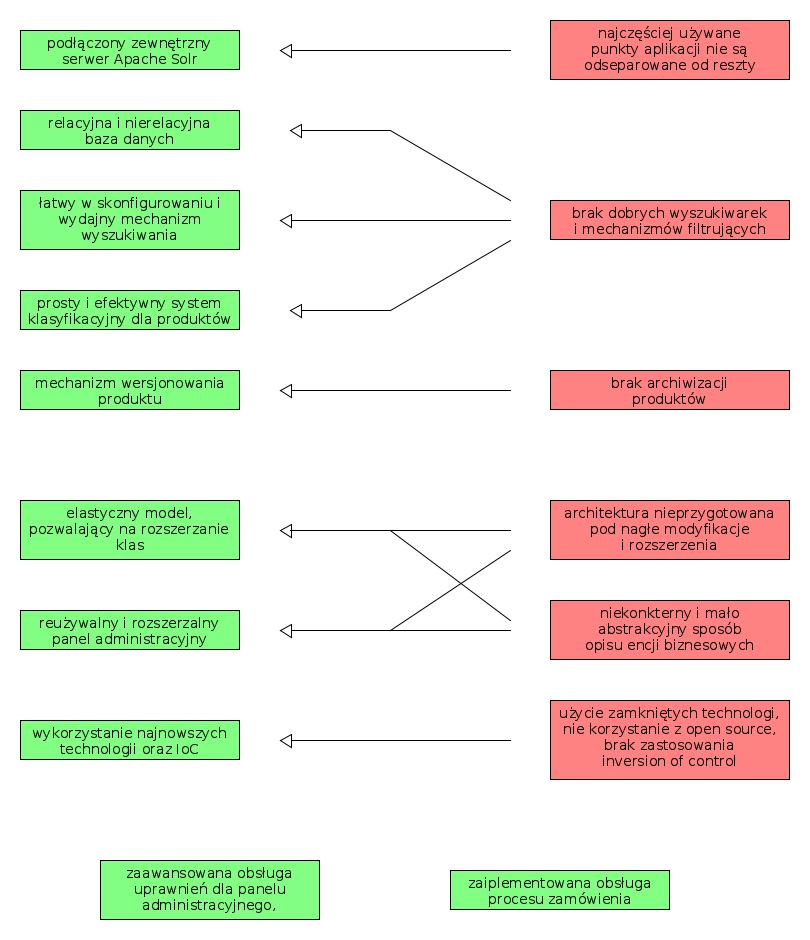
\includegraphics[width=1\textwidth]{wymagania.jpg}
	\end{center}
	\caption{{\color{dgray}Połączenie wymagań funkcjonalnych ze znalezionymi problemami.}} \label{wymagania}
\end{figure}

	\cleardoublepage

	\chapter{Projekt systemu}
\thispagestyle{chapterBeginStyle}

{\color{dgray}
W tym rozdziale przedstawiono szczegółowy projekt systemy w notacji UML uwzględniający wymagania funkcjonalne opisane w rozdziale~\ref{rozdzial1}. Do opisu relacji pomiędzy składowymi systemu wykorzystano diagramy \ldots.
Przedstawiono w pseudokodzie i omówiono algorytmy generowania \ldots.
}


\section{Grupy użytkowników i założenia}


\section{Przypadki użycia}
Jak zostało zdefiniowane w poprzednim punkcie, w pracy przewidziano 3 grupy użytkowników. W zamyśle framework jest narzędziem dla programisty, jednak w systemie został zaimplementowany szereg rozwiązań gotowych do wykorzystania dla końcowych użytkowników, dlatego diagramy przypadków użycia zostały podzielone na trzy klasy: 
\begin{itemize}
	\item przypadki użycia Programisty 
	\item przypadki użycia Użytkownika Administracyjnego potencjalnego serwisu e-commerce, opartego na opisywanym Frameworku
	\item przypadki użycia użytkownika końcowego, czyli Klienta
\end{itemize}
Na rysunku \ref{useCaseProgrammer} zostały przedstawione najważniejsze przypadki użycia frameworku. Programista ma swobodny dostęp do rozszerzania encji, w szczególności klasy Produkt, która ma wyjatkowo strategiczne znaczenie w systemach e-commerce. Dodatkowo ma możliwość uczynienia niestandardowych pól wyszukiwalnymi przez klienta. Sytuacja została zobrazowana na poniższym przykładzie.
\begin{example}
	Załóżmy, że mamy niestandardowe pole proste (String) w encji klasyfikowanej przez twórców ewentualnego sklepu związanego z opisywanym frameworkiem jako finalna encja nadająca się do sprzedaży. Niech nazywa się \texttt{MyProduct extends Product} z polem \texttt{myCustomField}. Jedyne co w tej sytuacji musimy zrobić aby system mógł wyciągnąć wartość tego pola z encji (o której de facto nie wie) to wpisać do tabeli zawierającej indeksowane cechy produktu nazwę danego pola, system za pomocą refleksji\footnote{\textit{refleksja} ( eng. reflection) -- udogodnienie w języku Java, pozwalające na wyświetlenie i manipulacje właściwościami klasy. Więcej w sekcji \textbf{słowniczek}.} wyekstaktuje wartość pola z encji.    
\end{example}
\begin{figure}
	\begin{center}
		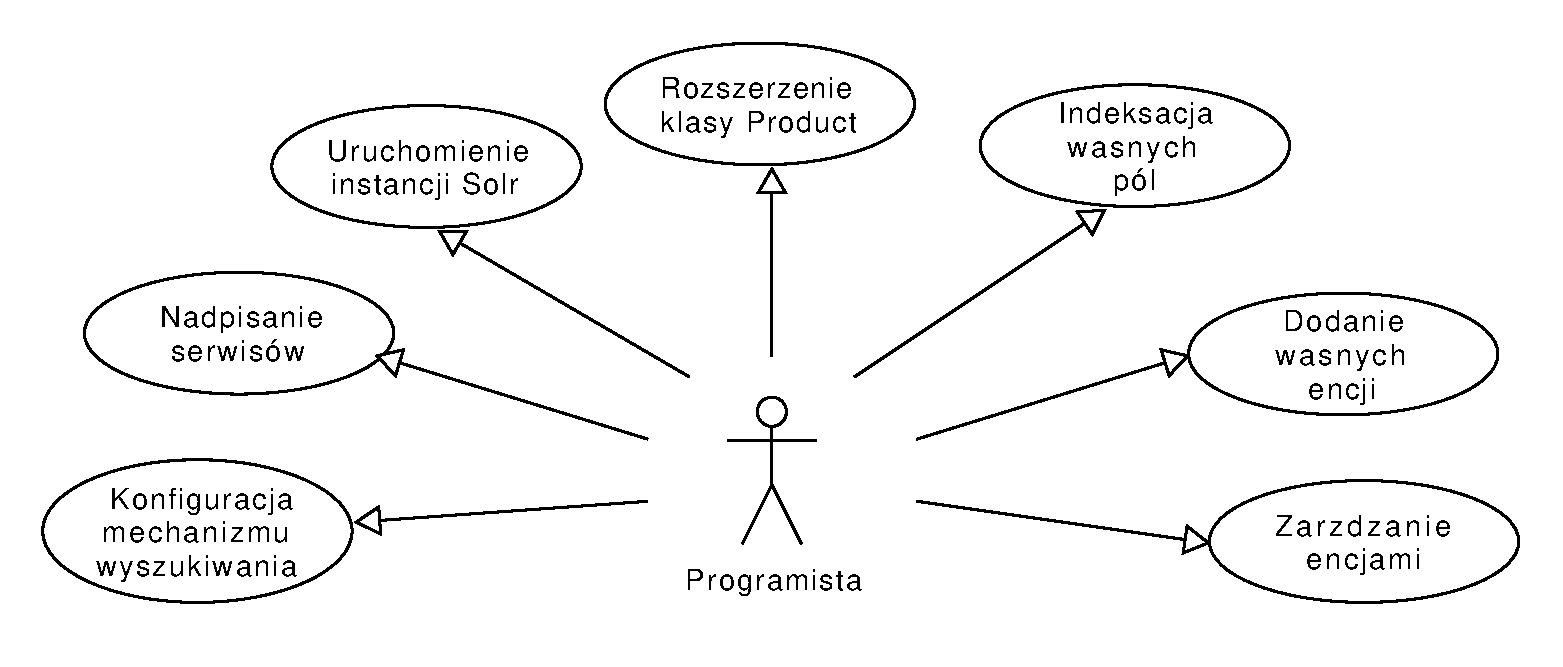
\includegraphics[width=1\textwidth]{ucdev.pdf}
	\end{center}
	\caption{{\color{black}Diagram przypadków użycia związany z Programistą.}} \label{useCaseProgrammer}
\end{figure}
\begin{figure}
	\begin{center}
		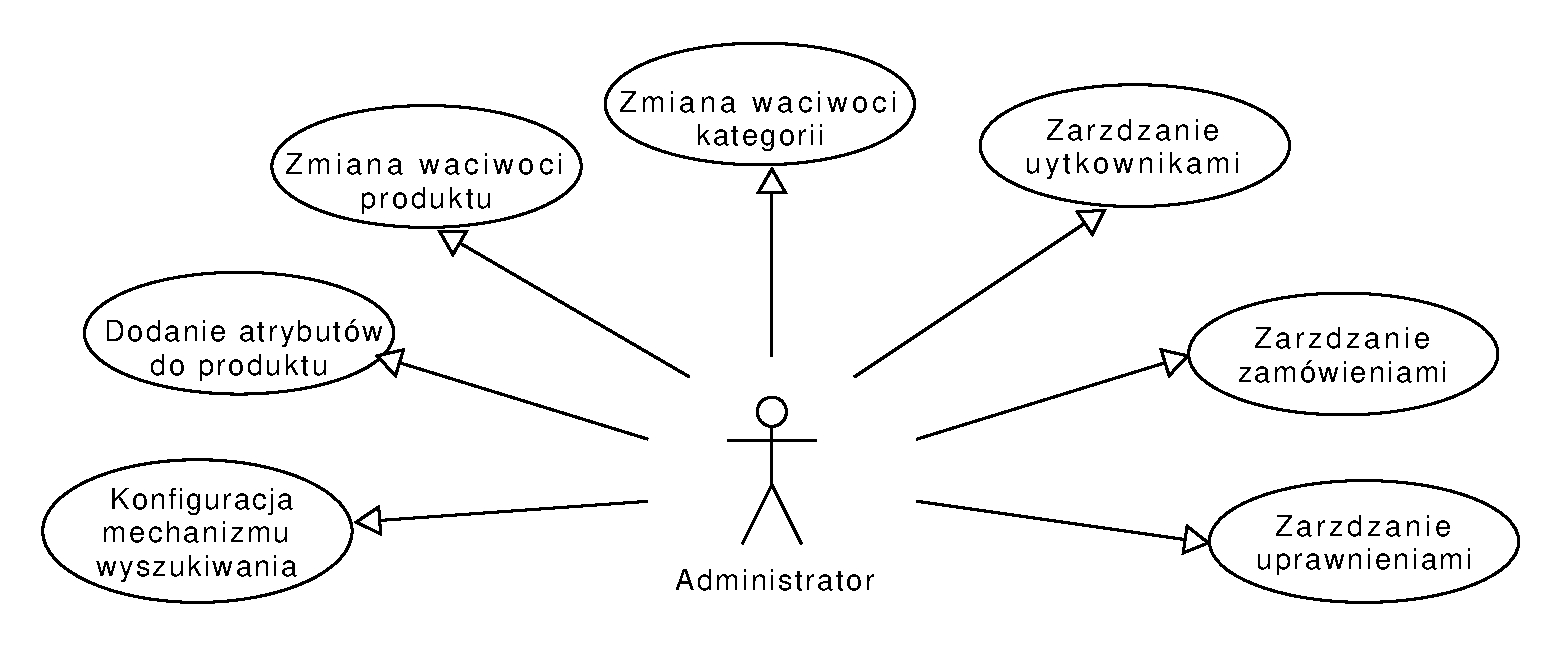
\includegraphics[width=1\textwidth]{ucadmin.pdf}
	\end{center}
	\caption{{\color{black}Diagram przypadków użycia związany z Administratorem ewentualniego systemu.}} \label{useCaseAdmin}
\end{figure}
Dodane przez Programistę encje są obsługiwane przez framework, dodatkowo po dodaniu specjalnej adnotacji\footnote{adnotacja -- używane w języku Java od wersji 1.7, najczęściej służą do określania dodatkowych właściwości pól bądź klas} nad nią, może być zarządzana w uniwersalnym panelu administracyjnym. Osoba zajmująca się implementacją sklepu opartego o opisywaną platformę może uruchomić dowolną \textit{(skończoną)} ilość instancji Apache Solr, czyli bazy danych noSQL, służącej do obsługiwania zapytań związanych z katalogiem produktowym (skalowalność pionowa tylko tej części aplikacji, która tego potrzebuje). W odniesieniu do przypadku użycia \textit{Nadpisanie mechanizmu wyszukiwania} z rysunku \ref{useCaseProgrammer} serwisy są oparte na interfejsach, zapewniając Programiście możliwość nadpisania jego logiki zgodnie z zasadami polimorfizmu. 

Rysunek \ref{useCaseAdmin} przedstawia przypadki użycia z punktu widzenia Administratora potencjalnego systemu. Z punktu widzenia platformy jest to również klient, gdyż framework zakłada, że nie ma on wiedzy technicznej i nie potrafi programować. Podobnie jak programista, może konfigurować mechanizm wyszukiwania, jednak bardziej wysokopoziomowo, np. deklaracja używanych facetów. Panel administracyjny zakłada zarządanie najważniejszymi encjami: produkt, kategoria, użytkownik, zamówienie, uprawnienie i parę innych, zdefiniowanych dokładniej w podrozdziale \textbf{Diagramy bazy danych}.

Diagram na rysunku \ref{useCaseCustomer} dotyczy przypadków użycia elementów frameworku przez końcowego użytkownika. Są to klasyczne funkcjonalności tradycyjnego sklepu internetowego. \textit{Wyszukanie produktu} zostało zaprojektowane, tak aby możliwy był również do zaimplementowania mechanizm podpowiedzi i podświetlania. Apache Solr udostępnia taką funkcjonalność. \textit{Reklamacja} dotyczy opisanego w rozdziale \textbf{Analiza problemu} kłopotu z archwizacją produktu, został on rozwiązany prostym mechanizmem wersjonowania. 
\begin{figure}[h!]
	\begin{center}
		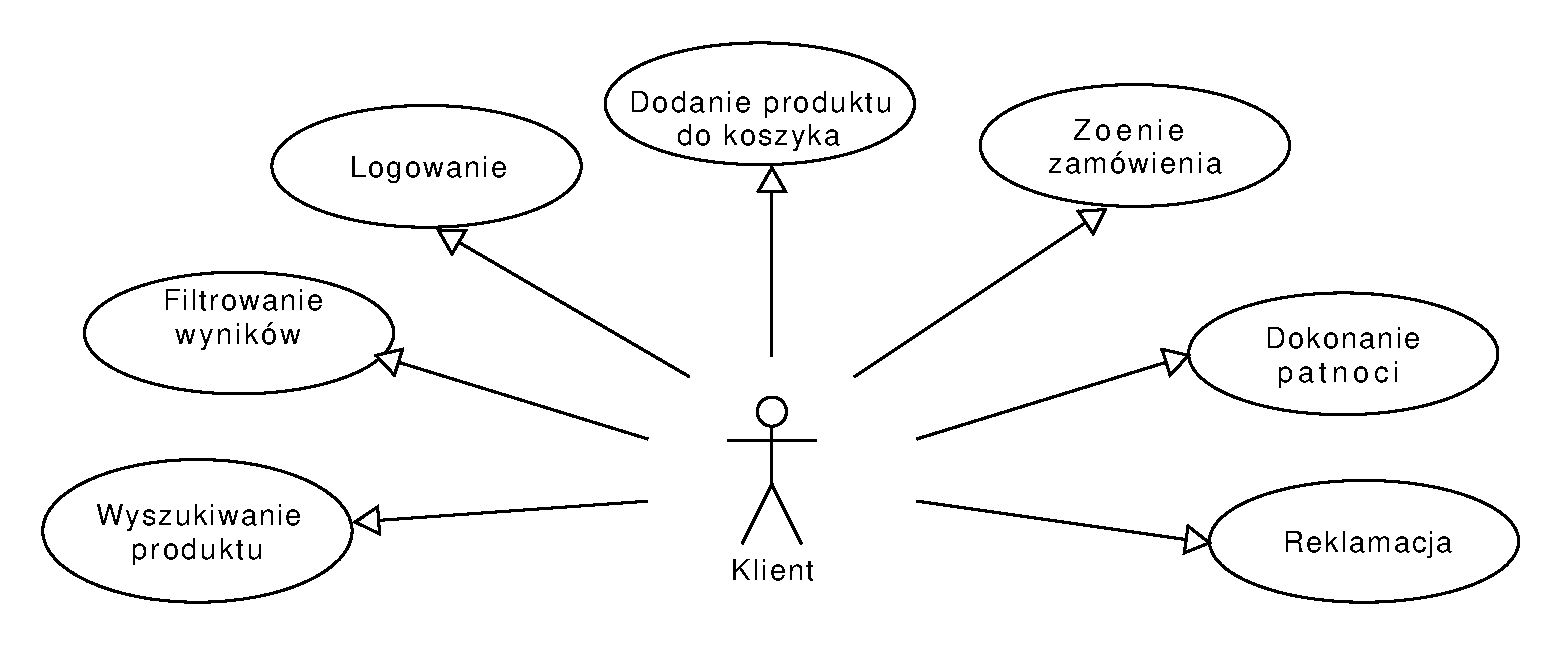
\includegraphics[width=1\textwidth]{uccustomer.pdf}
	\end{center}
	\caption{{\color{black}Diagram przypadków użycia związany z Administratorem ewentualniego systemu.}} \label{useCaseCustomer}
\end{figure}

\section{Diagramy klas}

W tej sekcji należy przedstawić diagramy klas dla odpowiednich elementów systemu zidentyfikowane na podstawie wcześniejszych rozważań

\section{Diagramy aktywności}

W tej sekcji należy przedstawić diagramy aktywności dla elementów systemu i odpowiednich procesów wynikające z wcześniejszej analizy.  

{\color{dgray}
W niniejszym rozdziale przedstawiono diagramy aktywności \ldots. Diagram na rysunku~\ref{czynnosci_GD} przedstawia \ldots.
} 

\begin{figure}[h!]
\begin{center}
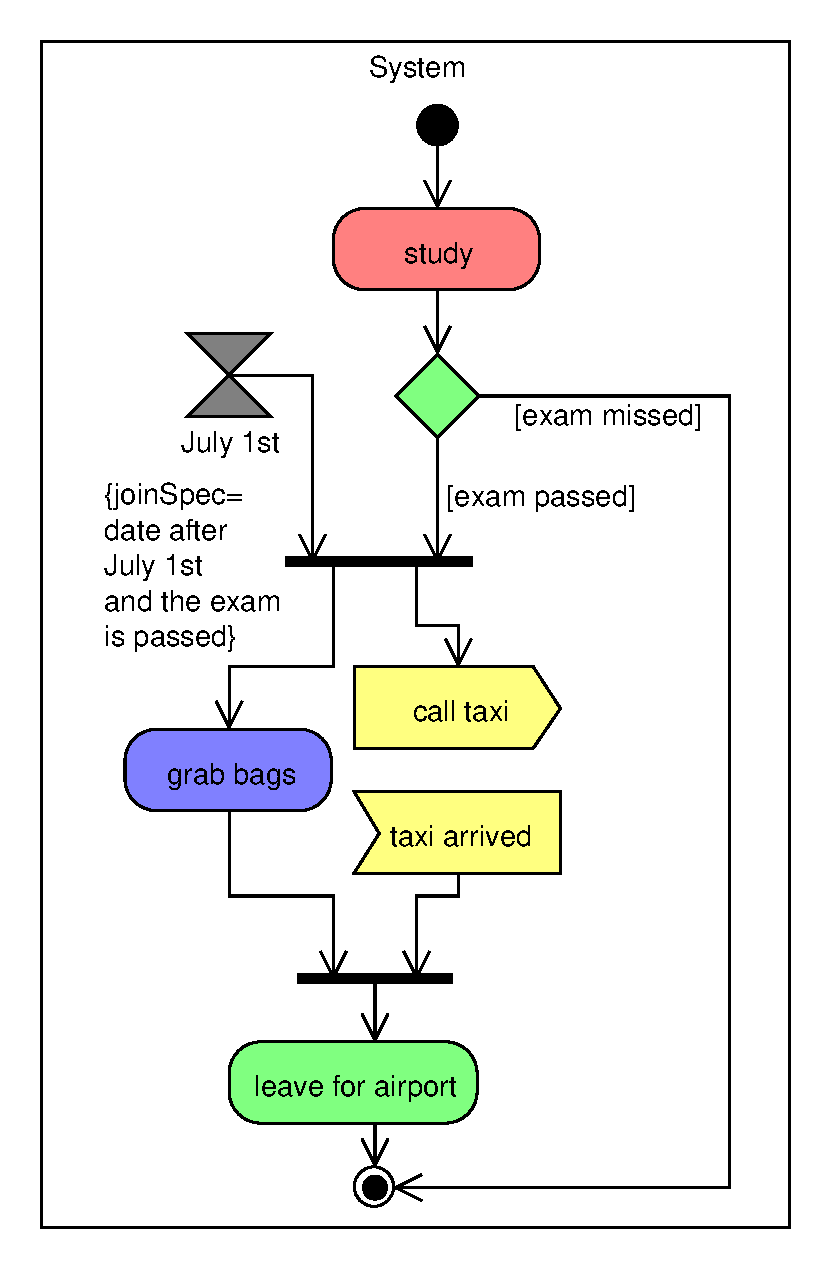
\includegraphics[width=0.5\textwidth]{aktyw.pdf}
\end{center}
\caption{{\color{dgray}Diagram aktywności związany z procesem rejestracji dokumentu.}} \label{czynnosci_GD}
\end{figure}  

\section{Diagramy sekwencji}

W tej sekcji należy przedstawić diagramy sekwencji dla obiektów systemu zidentyfikowanych na podstawie wcześniejszych rozważań. Należy wykorzystać nazewnictwo wprowadzone w poprzednich rozdziałach, w szczególności odpowiadające definicjom wprowadzonych klas.

\section{Diagramy stanów}

W tej sekcji należy przedstawić diagramy stanów w których może znaleźć się system. Diagramy te są szczególnie istotne przy projektowaniu systemów czasu rzeczywistego. 

\section{Projekt bazy danych}

W tej sekcji należy przedstawić projekt bazy danych. Należy omówić wycinek rzeczywistości i odpowiadające mu zidentyfikowane elementy systemu, których wartości będą podlegać utrwalaniu. Należy przedyskutować wybór typów danych dla atrybutów poszczególnych obiektów. Należy uzasadnić wybór platformy DBMS. Dla relacyjnych baz danych należy przedyskutować jej normalizację.

\section{Opis protokołów}

W tej sekcji należy omówić protokoły wykorzystywane przez komponenty systemu. Omówić formaty komunikatów i zilustrować je przykładami. 

\section{Opis algorytmów}

W tej sekcji należy wymienić i przedyskutować algorytmy wykorzystywane w systemie. Algorytmy należy przedstawić w pseudokodzie (wykorzystać pakiet \texttt{algorithm2e}). Omówienia poszczególnych kroków algorytmów powinny zawierać odwołania do odpowiednich linii pseudokodu. Dla zaproponowanych autorskich algorytmów należy przeprowadzić analizę ich złożoności czasowej i pamięciowej. 

{\color{dgray}
Algorytm bąblowania jest przedstawiony w Pseudokodzie~\ref{alg:mine}.
}

{\small
\begin{pseudokod}[H]
%\SetAlTitleFnt{small}
\SetArgSty{normalfont}
\SetKwFunction{Process}{Process}
\SetKwFunction{Calculate}{Calculate}
\KwIn{Zbiór bąbli $B$}
\KwOut{Wyporność $W$}
\ForEach{$b \in B$}{
\Process{$b$}\;
\For{$i \leftarrow 1$ \KwTo $|B|$}{
\If{\Calculate{EW($i$,$b$)} $\le$ 0}{
$b \leftarrow 2*b$\;
}
}
}
\While{$B \neq \emptyset$}{
\For{$j \leftarrow 1$ \KwTo $|B|$}{
\If{\Calculate{FT($j$,$\hat{b}$)} $\le 0$}{
$w \leftarrow 2*\hat{b}$\;
$W \leftarrow W \cup \{w\}$\;
$B \leftarrow B \setminus \{b\}$\;
}
}
}
\caption{Wyporność przez bąblowanie}\label{alg:mine}
\end{pseudokod}
}


	\cleardoublepage
	
	\chapter{Implementacja systemu}
\thispagestyle{chapterBeginStyle}

\section{Opis technologii}
W projektcie użyto wielu technologi oraz frameworków. Wszystkie oparte są o język Java, dokumentację można znaleźć w \cite{Java-doc}. Interfejs użytkownika zaprojektowano przy użyciu szablonów opartych o projekt Start Bootstrap, którego opis można znaleźć na stronie \cite{sb}. 

\subsection{Spring Framework/Spring Boot}
Główną technologią jest framework Spring. Ułatwia pisanie aplikacji w Javie, w szczególności webowych, ze względu na dużą elastyczność i wzorzec projektowy Model-View-Controller, singleton oraz spełnia zasadę \textit{Inversion of Control}. Aplikacja jest oparta o platformę Spring Boot. Jest to nakładka na framework Spring, który przy obecnych standardach stał się skomplikowany w konfiguracji. Spring Boot zapewnia autokonfigurację wielu komponentów systemu, łatwe dodawanie modułów Springowych (np. security lub web). Co najważniejsze posiada wbudowany kontener na aplikację internetową, przez co nie ma potrzeby konfigurowania osobnego kontenera (np. Tomcat) i umieszczania tam aplikacji. Znacznie przyśpiesza to dewelopment. Więcej informacji najduje się w dokumentacji \cite{springb-docs} oraz w książce \cite{springbook}.

\subsection{Hibernate/JPA 2.1} 
Java Persistence API jest interfejsem służącym do komunikacji aplikacji z bazą danych. Jego implementacją jest framework Hibernate. Korzystanie z tych standardów ułatwia komunikację z bazą danych i zapewnia wiele przydatnych funkcjonalności. Między innymi zapewnia również obsługę transakcji. W połączeniu ze Spring Data to potężne narzędzie, a jednocześnie jest proste w użytku. Więcej informacji o frameworku Hibernate i JPA w książce \cite{JPA-hib}. 
\subsection{Spring Data}
Spring Data ułatwia konfigurację połączeń między bazą danych, a serwerem. Do tego zapewnia automatyczne generowanie prostych kwerend bazodanowych, korzystając z zasady \textit{query by convention}\footnote{query by convention - sposób generowania kwerend bazodanowych na podstawie nazw metod w interfejsach}. Jest to sposób pisania nazw metod w interfejsach, które framework jest w stanie zaimplementować. Całość powoduje odejście tradycyjnej warstwy DataAccessObject. Framework pozwala na samodzielne implementowanie trudniejszych kwerend, w spersonalizowany sposób. 

\subsection{Apache Solr} 
Oparta na silniku Lucene i uruchomiona na osobnym serwerze wyszukiwarka zapewnia odseparowanie najbardziej obciążonej części sklepu. Dzięki Solrowi w implementowanym frameworku jest obecna bardzo szybka wyszukiwarka z możliwością wyszukiwania pełnotekstowego, filtrowania, sortowania i zawężania wyników względem różnych pól produktu. Książka \cite{solrbook} i dokumentacja \cite{Solr-doc} opisują działanie i możliwości Solra. Do integracji serwera Apache Solr z implementowanym frameworkiem użyto biblioteki SolrJ \cite{solrJ}.

\section{Omówienie kodów źródłowych}
Projekt składa się z 3986 linii kodu w języku Java, dlatego aby zachować zwięzłość i zrozumiałość w ramach omówienia kodów źródłowych zostanie przedstawiona tylko jedna funkcjonalność odnosząca się do konkretnych przypadków użycia zdefiniowanych w sekcji \textbf{Przypadki użycia} rozdziału \textbf{Projekt systemu}. 

Na rysunku \ref{useCaseProgrammer} znajduje się use-case: \textit{Zarządzanie encjami}. Związany jest przypadek z diagramu \ref{dynEntFormUC} \textit{Wyświetlenie i manipulacja relacjami encji}.  Te dwa przypadki wiążą się z konstrukcją dynamicznego formularza edycji dla danej encji. Dla lepszego zrozumienia warto przypomnieć diagramy związane z implementacją tej funkcjonalności. Na rysunku \ref{konsFormEnc} przedstawiono diagram aktywności, zaś rysunek \ref{klasy_formularz_encyjny} przedstawia klasy użyte do implementacji.

Dla przykładu działania kodu źródłowego zostanie przeanalizowana budowa formularza dla encji \texttt{Product}. Kod 

\begin{small}
\begin{lstlisting}[language=Java, frame=lines, numberstyle=\tiny, stepnumber=5, caption=Wyświetlenie formularza encyjnego: \texttt{DynamicEntityController.java}\label{ws}., firstnumber=1]


\end{lstlisting} 
\end{small}

{\color{dgray}
Kod źródłowy~\ref{req} przedstawia procedurę przetwarzającą żądanie. Hasz utrwalany \verb|%granulacja| wykorzystywany jest do komunikacji międzyprocesowej.
}https://docs.spring.io/spring-boot/docs/current/reference/htmlsingle/

\begin{small}
\begin{lstlisting}[language=perl, frame=lines, caption=Przetwarzanie żądania - procedura \texttt{process\_req()}\label{req}., firstnumber=86]
sub process_req(){	
  my($r) = @_;
  $wyn = "";
  if ($r=~/get/i) {
	@reqest = split(" ",$r);
	$zad = $reqest[0];
	$ts1 = $reqest[1];
	$ts2 = $reqest[2];
	@date1 = split(/\D/,$ts1);
	@date2 = split(/\D/,$ts2);
	print "odebralem: $r"; 
	$wyn = $wyn."zadanie: $zad\n";
	$wyn = $wyn."czas_od: "."$date1[0]"."-"."$date1[1]"."-"."$date1[2]"."_"."$date1[3]".":"."$date1[4]".":"."$date1[5]"."\n";
	$wyn = $wyn."czas_do: "."$date2[0]"."-"."$date2[1]"."-"."$date2[2]"."_"."$date2[3]".":"."$date2[4]".":"."$date2[5]"."\n";		
	$wyn = $wyn.&sym_sens($ts1,$ts2);
	return $wyn;
  }
  if ($r=~/set gt/i) {
	@reqest = split(" ",$r);
	$zad = $reqest[0];
	$ts1 = $reqest[1];
	$ts2 = $reqest[2];
	$gt = $reqest[2];
	dbmopen(%granulacja,"granulacja_baza",0644);
	$granulacja{"gt"}=$gt;
	dbmclose(%granulacja);
	$wyn = "\'GT\' zmienione na: $gt";
  }		
}	
\end{lstlisting} 
\end{small}

	\cleardoublepage
	
	\chapter{Wdrożenie i prezentacja działania}
\thispagestyle{chapterBeginStyle}

W tym rozdziale została przedstawiona instrukcja obsługi niniejszej platformy. W pierwszej części omówiono wymagania, które muszą zostać spełnione, aby framework z przykładowymi danymi był gotów do pracy, następnie opisano czynności instalacyjne. 
W dalszej części rozdziału umieszczono prezentację działania wybranych funkcjonalności, podzieloną ze względu na zdefiniowanych aktorów. 

%W tym rozdziale należy omówić zawartość pakietu instalacyjnego oraz założenia co do środowiska, w którym realizowany system będzie instalowany. Należy przedstawić procedurę instalacji i wdrożenia systemu. Czynności instalacyjne powinny być szczegółowo rozpisane na kroki. Procedura wdrożenia powinna obejmować konfigurację platformy sprzętowej, OS (np. konfiguracje niezbędnych sterowników) oraz konfigurację wdrażanego systemu, m.in.\ tworzenia niezbędnych kont użytkowników. Procedura instalacji powinna prowadzić od stanu, w którym nie są zainstalowane żadne składniki systemu, do stanu w którym system jest gotowy do pracy i oczekuje na akcje typowego użytkownika.%
\section{Wymagania początkowe}

\section{Instalacja aplikacji}

\section{Prezentacja wybranych funkcjonalności}

W ramach tej sekcji zostaną przedstawione najważniejsze funkcjonalności systemu, które pojawiły się w rozdziale \textbf{Projekt systemu}.  

\subsection{Funkcjonalności przewidziane dla administratora sklepu}
Sekcja ta ma za zadanie pokazać w praktyce deklarowaną wcześniej elastyczność systemu, czyli to,jak programista może skonfigurować platformę pod potrzeby sklepu, który implementuje.

\subsubsection{Widok panelu administracyjnego}
Na rysunku \ref{scr_adminmain} został przedstawiony panel administracyjny. Literkami A, B, C i D oznaczono ważne elementy. \textbf{A} -- konfigurowalne menu, \textbf{B} -- dynamiczna tabela encyjna ze wszystkim encjami rodzaju \texttt{price} (tabela cen). \textbf{C} przycisk dodania nowego egzemplarza encji, \textbf{D} -- linki z ID przekierowują do dynamicznego formularza edycji encji. 
\begin{figure}
	\begin{center}
		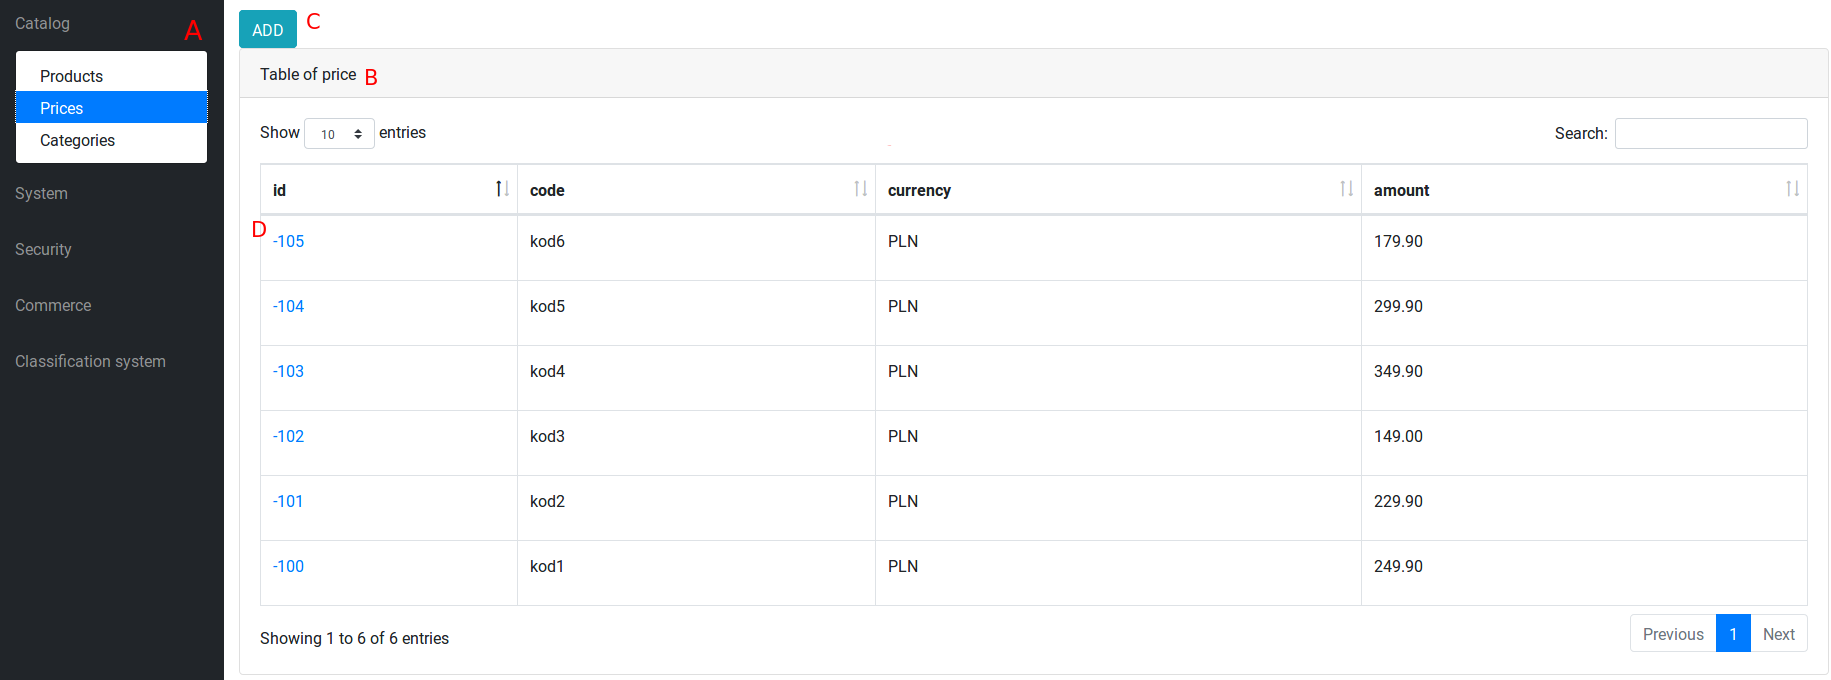
\includegraphics[width=1\textwidth]{admin-main.png}
	\end{center}
	\caption{{\color{black}Widok panelu administracyjnego}} \label{scr_adminmain}
\end{figure}

\subsubsection{Zmiana właściwości encji} 
Zmiana właściwości dowolnej encji zostanie przedstawiona na podstawie produktu.
 
\noindent
\textbf{Scenariusz: } zmiana ceny. \textbf{Rysunek: } \ref{zmianacenyproduktu} 
\begin{itemize}
	\item wybierz z tabeli encyjnej dowolny produkt i wejdź w szczegóły (1)
	\item w dynamicznym formularzu spośród relacji produktu wybierz cenę (price) i wejdź w szczegóły (2) 
	\item w formularzu edycji ceny zmień jej wartość i naciśnij \textit{submit}(3)
	\item po powrocie do edycji produktu zostanie wyświetlona zmieniona cena (4)
\end{itemize}
\begin{figure}
	\begin{center}
		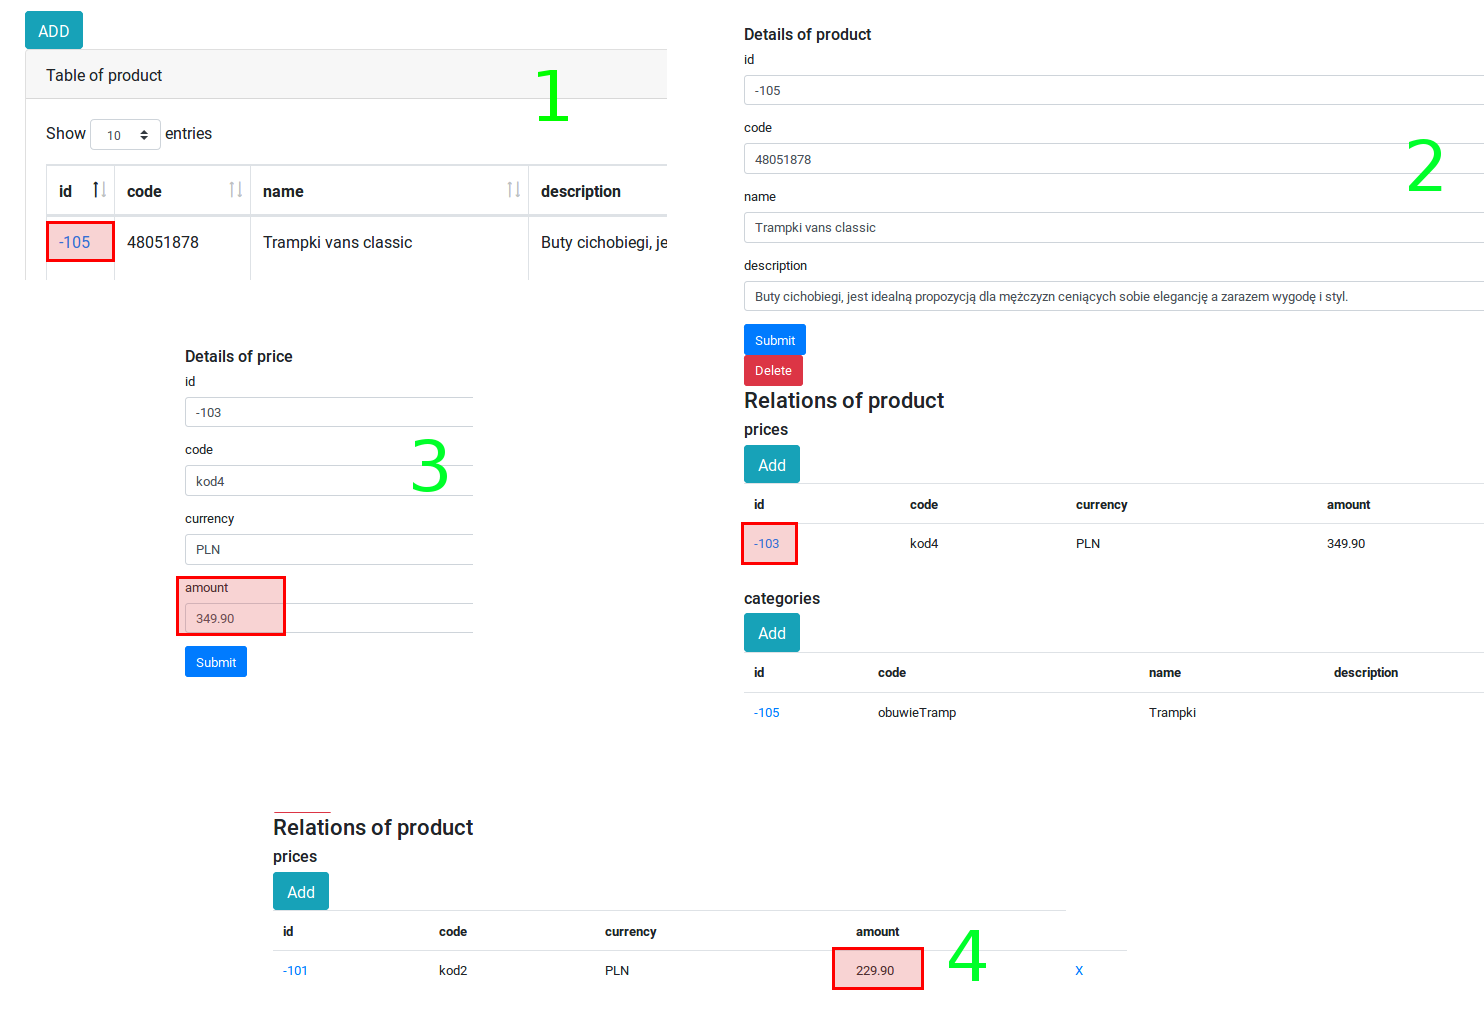
\includegraphics[scale=1.3]{zmianacenyproduktu.png}
	\end{center}
	\caption{{\color{black}Zmiana ceny w produkcie}} \label{zmianacenyproduktu}
\end{figure}


\subsection{Funkcjonalności przewidziane dla programisty}
Sekcja ta ma za zadanie pokazać w praktyce deklarowaną wcześniej elastyczność systemu, czyli to,jak programista może skonfigurować platformę pod potrzeby sklepu, który implementuje. 
\subsubsection{Dodanie encji do systemu}










	\cleardoublepage
	
	\chapter{Podsumowanie}
\thispagestyle{chapterBeginStyle}

Na podstawie niniejszej pracy został zaimplementowany szablonowy system, który pozwala na stworzenie sklepu internetowego opierającego się na gotowych rozwiązaniach. Wraz z platformą przychodzi szereg funkcjonalności, które są kluczowe dla każdego sklepu internetowego. 

Proces implementacji wiązał się z wieloma wyzwaniami. Najtrudniejszym z nich było stworzenie \textbf{elastycznego modelu}\footnote{spełnione wymagania funkcjonalne zdefiniowane w rozdziale \textbf{Analiza problemu} zostały wytłuszczone} oraz \textbf{reużywalnego i rozszerzalnego panalu administracyjnego}. Jest to jedno z ciekawszych rozwiązań, które pozwala na dowolną modyfikację modelu oraz wprowadzanie nowych funkcjonalności. Do systemu \textbf{podłączono zewnętrzny mechanizm indeksujący oraz relacyjną i nierelacyjną bazę danych}. Wraz z platformą użytkownicy mają do dyspozycji \textbf{zaawansowaną wyszukiwarkę Apache Solr}.

Do panelu administracyjnego dodano \textbf{funkcjonalność obsługi uprawnień} w obrębie użytkowników administracyjnych. Stworzono również \textbf{system klasyfikacyjny}, który umożliwia nadawanie dowolnych cech produktowi w zależności od kategorii, z której pochodzi. We frameworku został zaimplementowany także \textbf{pełny proces zakupowy} 

Wszystkie wymagania funkcjonalne określone we wstępie zostały spełnione, jednak biorąc pod uwagę charakter projektu, część z nich wymaga ciągłego udoskonalania. Platformy e-commerce są tworzone latami przez duże zespoły programistów, niemniej jednak projekt ten po dwumiesięcznym okresie implementacji można określić mianem konkretnego \textit{proof of concept}, który jest dobrym fundamentem do stworzenia bardzo dużego i jeszcze bardziej ogólnego rozwiązania. Warta przemyślenia byłby bardziej szczegółowy opis procesu zamówienia oraz, co byłoby bardzo praktyczne, to CMS, czyli system zarządzania treścią na sklepie, aby zapewnić możliwość edycji widoku sklepu z poziomu panelu administracyjnego. Interesującym pomysłem upraszczającym proces wdrożenia byłoby także zrobienie inicjalizera do projektów opartych na opisywanym frameworku, podobnego jak np. na stronie Spring Boot. 

Łącząc wszystkie zaimplementowane funkcjonalności w całość, otrzymamy system, który umożliwi nam szybką implementację sklepu internetowego. Dzięki tej pracy zaoszczędzony czas i pieniądze mogą zostać spożytkowane na lepszy marketing lub design. Taki był właśnie cel niniejszej pracy.  

	\cleardoublepage
	
	
	%%%%%%%%%%%%%%%%%%%%%%%%%%%%%%%%%%%%%%%%%%%%%%%%%%%%%%%%%%%%%%%%%%%%%%%%%%%%%%
	%%%%%%%%%%%%%%%%%%%%%%%%%%%%%%% BIBLIOGRAFIA %%%%%%%%%%%%%%%%%%%%%%%%%%%%%%%%%
	%%%%%%%%%%%%%%%%%%%%%%%%%%%%%%%%%%%%%%%%%%%%%%%%%%%%%%%%%%%%%%%%%%%%%%%%%%%%%%

	\pagestyle{bibliographyStyle}
	\bibliographystyle{plabbrv}
	\bibliography{literatura}
	\thispagestyle{chapterBeginStyle}
        \addcontentsline{toc}{chapter}{Bibliografia}

	\cleardoublepage
	
	%%%%%%%%%%%%%%%%%%%%%%%%%%%%%%%%%%%%%%%%%%%%%%%%%%%%%%%%%%%%%%%%%%%%%%%%%%%%%%
	%%%%%%%%%%%%%%%%%%%%%%%%%%%%%%%%% DODATKI %%%%%%%%%%%%%%%%%%%%%%%%%%%%%%%%%%%%
	%%%%%%%%%%%%%%%%%%%%%%%%%%%%%%%%%%%%%%%%%%%%%%%%%%%%%%%%%%%%%%%%%%%%%%%%%%%%%%
	
	\appendix
	\pagestyle{appendixStyle}
	
	\chapter{Zawartość płyty CD}
\thispagestyle{chapterBeginStyle}
\label{plytaCD}

Płyta CD zawiera pakiet instalacyjny dla testowej aplikacji. Główny katalog ma w sobie dwa podkatalogi \texttt{sql i tine-commerce}, ten pierwszy zawiera pliki sql z poleceniami tworzącymi bazę danych oraz testowe dane. Folder \texttt{tine-commerce} zawiera kod źródłowy platformy. W głównym katalogu są również dwa pliki \texttt{.jar}: \texttt{admin.jar i shop.jar}, które składają się na przykładową aplikację (sklep internetowy wraz z panelem administracyjnym). Na płycie CD znajduje się także niniejsza praca w pliku o nazwie \texttt{W11\_229773\_2019\_praca\_inżynierska.pdf}.


	\cleardoublepage

\end{document}

